\section{Experiments and Results}
\label{experiments}

  %测试的benchmark，使用什么样的LLM大模型，强化学习的模型，
%关于数据部分的模型，做SFT和RL的模型，不同系列的开源模型，同一模型的不同scale模型。做SFT的配置，强化学习的算法等配置
% 模型角度：
% 1. 语料库构造使用的模型
% 2. SFT和RL的模型
% 3. 消融实验的模型：不同系列的开源模型，同一模型的不同scale模型
% 实验配置角度
% 4. SFT 配置 
% 5. RL 配置 （不同的数据组合方式）
\subsection{Experimental Setups}

\begin{comment}

\textbf{Models.}
As summarized in Table~\ref{tab:models_training}, we employ different large language models at each stage according to their respective roles. 
For dataset construction, {DeepSeek-R1}~\cite{abs250112948} is used for document-based data generation and single-file Chain-of-Thought (CoT) construction (Secs.~\ref{document_dataset} and~\ref{single_file}). 
To support project-level CoT construction that requires reasoning over complete kernel projects with multiple mutually referenced source files, we adopt {Gemini 2.5 Pro}~\cite{google_gemini_2_5_pro} (Sec.~\ref{project_file}), which owing to its stronger support for multi-file code understanding and cross-file dependency reasoning. 
Within the data flywheel in SFT (Secs.~\ref{sft_api_correction} and~\ref{sft_kernel_correction}), {DeepSeek-Reasoner} is further leveraged to iteratively refine and correct the generated reasoning chains.

\end{comment}

\textbf{Models.}
As summarized in Table~\ref{tab:models_training}, we employ different large language models at distinct stages of the pipeline according to their functional roles. For dataset construction and document-level reasoning, we adopt DeepSeek-R1~\cite{abs250112948}, which is used to generate document-based data and single-file Chain-of-Thought (Secs.~\ref{document_dataset} and~\ref{kernel_dataset}). For project-level reasoning that requires understanding multi-file kernel implementations with cross-file dependencies, we employ Gemini~2.5~Pro~\cite{google_gemini_2_5_pro}, leveraging its stronger support for long-context and multi-file code reasoning (Sec.~\ref{kernel_dataset}). Within the supervised fine-tuning (SFT) data, DeepSeek-Reasoner is further used to iteratively refine and correct reasoning traces (Secs.~\ref{sft_api_correction} and~\ref{sft_kernel_correction}).

%For model training, we adopt \textbf{Qwen3-32B}~\cite{qwen3technicalreport} as the backbone model for supervised fine-tuning (SFT) and reinforcement learning (RL). 
%To study the effect of model scale and architecture, we additionally conduct SFT on multiple Qwen variants, including Qwen3-1.7B, 4B, 8B, 14B, and 32B, as well as the code-specialized Qwen3-Coder-30B-A3B-Instruct.

% \noindent\textbf{Training} 
% % SFT 
% % RL 
% To effectively inject kernel-specific knowledge into the LLM, we adopt a two-stage training strategy. 
% The first stage performs SFT on the AscendC dataset constructed as described in Sec.~\ref{data_construct}, which consists of three categories: AscendC document data, AscendC kernel data, and general reasoning chains. 
% To evaluate the contribution of each category, we conduct ablation studies by removing one component at a time. 
% We also assess the impact of data scale by performing SFT with 25\%, 50\%, and 75\% of the dataset.
% The second stage is reinforcement learning (RL), we adopt Direct Preference Optimization~(DPO) \cite{RafailovSMMEF23} with a learning rate of $1\times10^{-6}$, cosine learning rate decay, and a warm-up ratio of 0.1. The global batch size is set to 64, the training runs for 150 iterations, and the DPO loss uses a sigmoid formulation with $\beta=0.1$. We also analysis different positive/negative pairs for this training preference dataset.
% We further analyze the impact of different positive and negative sample selection strategies in constructing the preference dataset Sec. \ref{reinforcement_learning} for reinforcement learning.

\begin{comment}

\noindent\textbf{Training.}
We adopt a two-stage training strategy consisting of supervised fine-tuning~(SFT) followed by reinforcement learning~(RL). 
In the first stage, SFT is performed using {Qwen3-32B}~\cite{qwen3technicalreport} as the backbone model. 
To analyze the effect of model scale and architecture, we additionally conduct SFT on multiple Qwen variants, including Qwen3-1.7B, 4B, 8B, 14B, and 32B, as well as the code-specialized Qwen3-Coder-30B-A3B-Instruct. 
All SFT experiments are conducted under a unified training setup, with comparisons between full fine-tuning and LoRA-based tuning following the configurations summarized in Table~\ref{tab:models_training}.
In the second stage, RL is conducted using {Direct Preference Optimization} (DPO)~\cite{RafailovSMMEF23} under a fixed training configuration. 
Specifically, we use a learning rate of $1\times10^{-6}$ with cosine decay and a warm-up ratio of 0.1, a global batch size of 64, and train for 150 iterations. 
We further analyze the impact of different positive and negative sample selection strategies in constructing the preference dataset, as detailed in Sec.~\ref{reinforcement_learning}.

\end{comment}

\textbf{Training.}
We adopt a two-stage training strategy consisting of supervised fine-tuning followed by reinforcement learning. In the SFT stage, Qwen3-32B~\cite{qwen3technicalreport} serves as the primary backbone model. To analyze the impact of model scale and architecture, we additionally conduct SFT on multiple Qwen variants ranging from 1.7B to 32B parameters, as well as the code-specialized Qwen3-Coder-30B-A3B-Instruct. All SFT experiments share a unified training configuration, with both full fine-tuning and LoRA-based tuning evaluated under controlled settings (Table~\ref{tab:models_training}). In the second stage, reinforcement learning is performed using Direct Preference Optimization (DPO)~\cite{RafailovSMMEF23}, with detailed configurations and ablation studies reported in Sec.~\ref{reinforcement_learning}.

\begin{table}[t]
\centering
\caption{Overview of models and configurations used for dataset construction and two-stage training.}
\label{tab:models_training}
\resizebox{0.9\linewidth}{!}{
\begin{tabular}{p{3.7cm} p{3.9cm} p{3.9cm} p{5.5cm}}
\toprule
\textbf{Stage} & \textbf{Model / Method} & \textbf{Role} & \textbf{Description} \\
\midrule

\multirow{9}{*}{Dataset Construction} %9代表description有9个物理行
& DeepSeek-R1
& Document \& Single-file CoT 
& Document-based data generation and single-file Chain-of-Thought construction \\

& Gemini 2.5 Pro
& Project-level CoT 
& Reasoning over complete kernel projects with multiple mutually referenced source files \\

& DeepSeek-Reasoner 
& Data Flywheel Refinement
& Iterative correction and refinement of generated reasoning chains within the data flywheel \\
\midrule

\multirow{10}{*}{Supervised Fine-tuning}  %10代表description列有10个物理行
& Qwen3-32B
& Backbone Model 
& Backbone model for supervised fine-tuning \\

& Qwen3-1.7B / 4B / 8B / 14B / 32B / Coder-30B-A3B-Instruct 
& Scaling Study 
& Supervised fine-tuning across different model scales and architectures \\

& Training Configuration 
& Full FT / LoRA 
& Learning rate $1.25\times10^{-6}$ (Full FT) vs. $1.25\times10^{-5}$ (LoRA), cosine decay, warm-up ratio 0.01, micro/global batch size 1/128, weight decay $1\times10^{-1}$, gradient clipping 1.0. \\

\midrule

\multirow{7}{*}{Reinforcement Learning}  %7代表description列有7个物理行
& DPO
& Optimization Objective 
& Direct Preference Optimization with $\beta=0.1$ \\

& Training Configuration 
& Hyperparameters 
& Learning rate $1\times10^{-6}$, cosine decay, warm-up ratio 0.1, global batch size 64, 150 training iterations \\

& Preference Construction 
& Ablation Analysis 
& Analysis of different positive and negative sample selection strategies \\
\bottomrule
\end{tabular}}
\end{table}


\subsection{NPUKernelBench and Evaluation Metrics} % 测试的算子介绍，评价指标编译和精度

\begin{comment}

Our evaluation is conducted on \textbf{NPUKernelBench}, as introduced in Sec.~\ref{NPUKernelBench}. 
It consists of 158 representative CANN kernels organized into three levels of computational complexity, each accompanied by a reference Python implementation with standardized input/output specifications for automated evaluation.
For each kernel, we generate AscendC code using the evaluated LLM and subsequently compile and execute the generated kernels on the target NPU platform. To assess the robustness and scalability of the generated kernels, we evaluate each task under \textbf{multiple input data sizes}, as summarized in Table xxx. This setting allows us to examine the model's generalization ability across varying workload intensities and input scales.
% \paragraph{Evaluation Metrics.}
We adopt two complementary metrics to comprehensively evaluate the quality of generated kernels:

\begin{itemize}
    \item \textbf{Compilation Rate.}  
    This metric measures whether a generated AscendC kernel can be successfully compiled by the CANN toolchain without errors. 
    A kernel is considered \emph{successfully compiled} only if it passes the full compilation process, reflecting the model's ability to generate valid and API-compliant kernel code.

    \item \textbf{Execution Rate.} 
    For kernels that compile successfully, Execution Rate is evaluated by comparing their outputs with the reference Python implementations under a predefined numerical tolerance. We additionally report correctness for different kernel complexity levels, as described in Sec.~\ref{kernelbench_correctness}.

    \item \textbf{Performance Speedup.}  This metric evaluates the runtime efficiency of generated kernels by comparing their average execution time with expert-implemented kernels. For each kernel, we compute the \emph{Speedup} as $\text{Speedup} = T_{\text{expert}} / T_{\text{gen}}$, where $T_{\text{expert}}$ and $T_{\text{gen}}$ denote the average execution time of expert-implemented and generated kernels, respectively; values greater than $1.0$ indicate performance improvement, while values below $1.0$ imply a slowdown.

\end{itemize}

\end{comment}

All evaluations are conducted on NPUKernelBench (Sec.~\ref{NPUKernelBench}), which contains 158 representative kernels spanning three levels of computational complexity.
Each kernel is accompanied by a reference implementation with standardized input and output specifications, enabling automated correctness verification.

For each task, we generate kernel code using the evaluated LLM and execute the compiled kernels on the target NPU platform. To assess robustness and scalability, each kernel is evaluated under multiple input sizes, allowing us to examine generalization behavior across varying workload intensities.

We evaluate generated kernels along three complementary dimensions. First, the \emph{Compilation Rate} measures whether a kernel can be successfully compiled, reflecting syntactic validity and API compliance; this metric is reported as pass@$k$, indicating the fraction of tasks for which at least one of the top-$k$ generated candidates compiles successfully. Second, the \emph{Execution Rate} assesses functional correctness by comparing kernel outputs against reference implementations under predefined numerical tolerances (Sec.~\ref{kernelbench_correctness}), and is likewise measured under the pass@$k$ protocol. Finally, \emph{Performance Speedup} evaluates runtime efficiency by normalizing kernel latency against expert-implemented baselines, with values greater than one indicating performance improvements.


\subsection{Main Results} %实验结果比较，未经sft的，sft，强化学习的

We compare kernel generation performance across different training stages, including the base models, supervised fine-tuning, and reinforcement learning. Overall, performance improves consistently as training progresses, with increasingly robust behavior observed on more challenging kernels. Quantitative results under different sampling budgets are summarized in Table~\ref{tab:pass_k_results_speed} and analyzed in detail below.

% \begin{table}[t]
%     \centering
%     \small
%     \renewcommand{\arraystretch}{1.1} % 稍微调整行高
    
%     % 总标题
%     \caption{Evaluation results of kernel generation on NPUKernelBench across different sampling budgets ($k$). We report Compile Rate (CR), Execution Success Rate (ESR), and Speedup for Pass@1, Pass@10, and Pass@100.}
%     \label{tab:pass_k_results}

%     % --- 子表 (a): Pass@1 ---
%     \begin{subtable}{1\linewidth}
%         \centering
%         \caption{Results for \textbf{Pass@1}}
%         \begin{tabular}{l cc c c}
%             \toprule
%             \textbf{Model} & \textbf{Level} & \textbf{Compile Rate (\%)} & \textbf{Exec. Rate (\%)} & \textbf{Speedup ($\times$)} \\
%             \midrule
%             \multirow{2}{*}{QWen3-32B}      & Level 1    & 38.08 & 17.39 & 0.85 \\
%             & Level 2    & 0.0 & 0.0 &  - \\ 
%             & Mean       & 45.72 & 11.59 & - \\ 

%             \multirow{2}{*}{QWen3-32B + SFT}  & Level 1       & 60.5 & 28.1 & 0.95 \\
%             & Level 2    & 52.4 & 21.5 & 0.85 \\ 
%             & Mean       & 52.4 & 21.5 & 0.85 \\ 
%             \multirow{2}{*}{QWen3-32B + SFT + RL}   & Level 1      & 60.5 & 28.1 & 0.95 \\
%             & Level 2    & 52.4 & 21.5 & 0.85 \\ 
%             & Mean       & 52.4 & 21.5 & 0.85 \\ 
%             \bottomrule
%         \end{tabular}
%         \label{subtab:pass1}
%     \end{subtable}
    
%     \bigskip % 添加垂直间距

%     % --- 子表 (b): Pass@10 ---
%     \begin{subtable}{1\linewidth}
%         \centering
%         \caption{Results for \textbf{Pass@10}}
%         \begin{tabular}{l cc c c}
%             \toprule
%             \textbf{Model} & \textbf{Level} & \textbf{Compile Rate (\%)} & \textbf{Exec. Rate (\%)} & \textbf{Speedup ($\times$)} \\
%             \midrule
%              \multirow{2}{*}{QWen3-32B}      & Level 1    & 52.4 & 21.5 & 0.85 \\
%             & Level 2    & 52.4 & 21.5 & 0.85 \\ 
%             & Mean       & 52.4 & 21.5 & 0.85 \\ 
%             \multirow{2}{*}{QWen3-32B + SFT}  & Level 1       & 60.5 & 28.1 & 0.95 \\
%             & Level 2    & 52.4 & 21.5 & 0.85 \\ 
%             & Mean       & 52.4 & 21.5 & 0.85 \\ 
%             \multirow{2}{*}{QWen3-32B + SFT + RL}   & Level 1      & 60.5 & 28.1 & 0.95 \\
%             & Level 2    & 52.4 & 21.5 & 0.85 \\ 
%             & Mean       & 52.4 & 21.5 & 0.85 \\ 
%             \bottomrule
%         \end{tabular}
%         \label{subtab:pass10}
%     \end{subtable}

%     \bigskip % 添加垂直间距

%     % --- 子表 (c): Pass@100 ---
%     \begin{subtable}{1\linewidth}
%         \centering
%         \caption{Results for \textbf{Pass@100}}
%         \begin{tabular}{l cc c c}
%             \toprule
%             \textbf{Model} & \textbf{Level} & \textbf{Compile Rate (\%)} & \textbf{Exec. Rate (\%)} & \textbf{Speedup ($\times$)} \\
%             \midrule
%              \multirow{2}{*}{QWen3-32B}      & Level 1    & 52.4 & 21.5 & 0.85 \\
%             & Level 2    & 52.4 & 21.5 & 0.85 \\ 
%             & Mean       & 52.4 & 21.5 & 0.85 \\ 
%             \multirow{2}{*}{QWen3-32B + SFT}  & Level 1       & 60.5 & 28.1 & 0.95 \\
%             & Level 2    & 52.4 & 21.5 & 0.85 \\ 
%             & Mean       & 52.4 & 21.5 & 0.85 \\ 
%             \multirow{2}{*}{QWen3-32B + SFT + RL}   & Level 1      & 60.5 & 28.1 & 0.95 \\
%             & Level 2    & 52.4 & 21.5 & 0.85 \\ 
%             & Mean       & 52.4 & 21.5 & 0.85 \\ 
%             \bottomrule
%         \end{tabular}
%         \label{subtab:pass100}
%     \end{subtable}
% \end{table}
\begin{table}[t]
\centering
\small
\renewcommand{\arraystretch}{1.1}
\caption{Evaluation results of kernel generation on NPUKernelBench across different sampling budgets ($k$). We report Compilation Rate (CR), Execution Rate (ER), and overall Speedup for generated kernels.}
\label{tab:pass_k_results_speed}
\resizebox{1\linewidth}{!}{
\begin{tabular}{l c cc cc cc c}
\toprule
\multirow{2}{*}{\textbf{Model}} & \multirow{2}{*}{\textbf{Level}} & \multicolumn{2}{c}{\textbf{Pass@1}} & \multicolumn{2}{c}{\textbf{Pass@10}} & \multicolumn{2}{c}{\textbf{Pass@100}} & \multirow{2}{*}{\textbf{Speedup ($\times$)}} \\
\cmidrule(r){3-4} \cmidrule(r){5-6} \cmidrule(r){7-8}
 & & CR (\%) & ER (\%) & CR (\%) & ER (\%) & CR (\%) & ER (\%) &  \\
\midrule
\multirow{4}{*}{Qwen3-32B} & Level 1 & 38.08 & 17.39 &71.62  &48.84  &75.00  &66.67  & 0.60 \\
 & Level 2 & 0.0 & 0.0 & 0.0 & 0.0 & 0.0 & 0.0 & 0.0 \\
 & Level 3 & 1.83 & 0.0 & 15.43 & 0.0 & 50.00 & 0.0 & 0.0 \\
 \rowcolor{bggreen}
 & Mean & 25.59 &11.59  & 49.46 & 32.56 & 55.56 & 44.44 & 0.60 \\
\midrule
\multirow{4}{*}{Qwen3-32B + SFT} & Level 1 &84.83  &38.28  &99.97  &86.82  &100  &94.44  & 0.56 \\
 & Level 2 &60.5 &8  &96.54  &40.48  &100 &75  & 1.50 \\
 & Level 3 &17 &0.17  &63.75  &1.67  &100 &16.67  & 0.00 \\
 \rowcolor{bggreen}
 & Mean &\textbf{71.89}  &27.31  &\textbf{95.18}  &67.06 &\textbf{100} & 81.48 &  0.75 \\
\midrule
\multirow{4}{*}{Qwen3-32B + SFT + RL} & Level 1 &82.17 &43.28 &99.92 &93.89 &100 &100 & 0.61 \\
 & Level 2 &62.75 &14.25 &95.49 &64.28 &100 &91.67 & 1.86 \\
 & Level 3 &14.67 &0.17  &61.12  &1.67  &100 &16.67  & 0.00 \\
 \rowcolor{bggreen}
 & Mean &70.35 &\textbf{32.04} &94.62 &\textbf{77.06} &\textbf{100} &\textbf{88.89} & 0.87 \\

\bottomrule
\end{tabular}}
\end{table}



\begin{figure*}
    \centering
    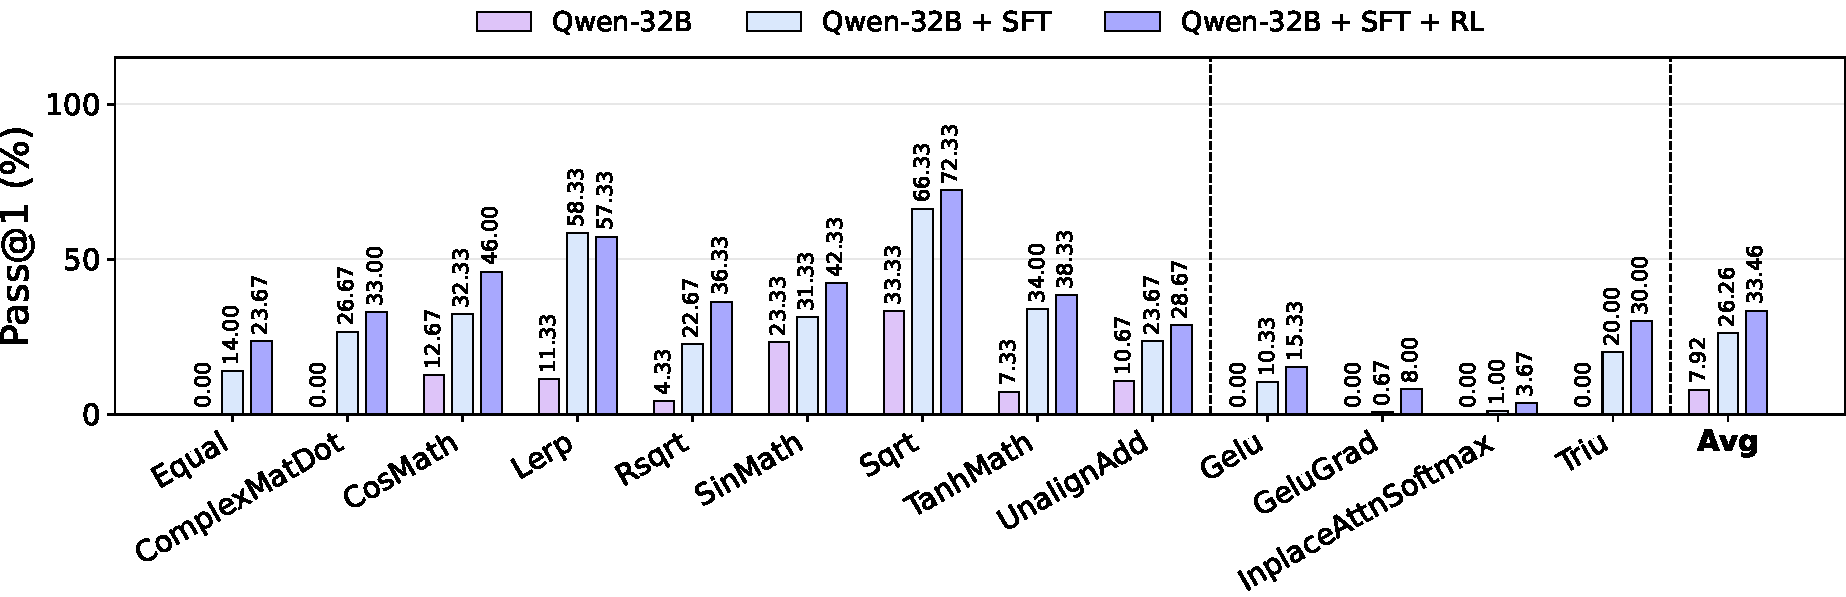
\includegraphics[width=0.98\linewidth]{pdfs/level1_level2_Avg_pass1.pdf}
    %\caption{Kernel-wise Pass@1 performance comparison of selected operators across training stages. This bar chart visualizes the accuracy of chosen kernels from Qwen-32B across Base, SFT, and RL stages. While all models show improved performance, RL particularly enhances accuracy for complex kernels, allowing for a comparative analysis of their effectiveness at each stage.}
    \caption{Pass@1 results for representative kernels across training stages.}
    \label{fig:Specific_kernel_acc}
\end{figure*}

\subsubsection{Compilation and Execution}

\begin{comment}

Table~\ref{tab:pass_k_results_speed} reports the evaluation results of kernel generation on NPUKernelBench under different sampling budgets ($k$) and difficulty levels. We observe a clear correlation between kernel difficulty and generation performance. For the base QWen3-32B model, Level 1 kernels achieve moderate Compile Rate (CR) and Execution Success Rate (ER), while Level 2 kernels are largely unsolved and Level 3 kernels show very low ER despite some improvements in CR at higher $k$. Incorporating supervised fine-tuning (SFT) substantially boosts both CR and ER across all levels, especially for Level 1 and Level 2 kernels, indicating that SFT helps the model better capture task-specific patterns. Further enhancement with reinforcement learning (RL) yields additional gains in ER, particularly for higher difficulty levels, suggesting that RL effectively guides the model toward more executable kernels. Overall, the mean performance demonstrates that hierarchical training strategies (SFT + RL) significantly improve kernel generation quality and robustness across varying kernel difficulty levels, while also achieving notable speedup in execution.

\end{comment}

Table~\ref{tab:pass_k_results_speed} summarizes kernel generation performance on NPUKernelBench across different sampling budgets ($k$) and difficulty levels.
A clear performance gap emerges as kernel complexity increases.
For the base Qwen3-32B model, Level~1 kernels achieve moderate compilation rates (CR) and execution success rates (ER), whereas Level~2 kernels remain largely unsolved.
For Level~3 kernels, although higher $k$ improves CR to some extent, ER remains consistently low, indicating that successful compilation alone does not guarantee correct execution for complex kernels.

Figure~\ref{fig:Specific_kernel_acc} presents the Pass@1 accuracy of Qwen-32B on a set of representative kernels across three training stages: the base model, supervised fine-tuning (SFT), and SFT followed by reinforcement learning (RL).
The base model exhibits limited kernel synthesis capability, achieving an average Pass@1 of only 7.92\%, which reflects the difficulty of directly transferring general-purpose code generation ability to low-level NPU kernel programming.

Supervised fine-tuning leads to a substantial improvement, increasing the average Pass@1 to 26.26\%.
This gain indicates that SFT effectively aligns the model with the structural and syntactic requirements of kernel generation, enabling it to produce compilable and partially correct implementations.
In particular, SFT equips the model with essential building blocks such as API usage patterns, memory object initialization, and canonical computation templates, which are prerequisites for valid kernel synthesis.

Building upon this foundation, reinforcement learning further improves the average Pass@1 accuracy to 33.46\%.
Unlike SFT, which primarily addresses coarse-grained correctness, RL provides execution-based preference signals that encourage the model to distinguish between multiple valid but semantically different implementations.
The resulting improvements are especially pronounced for complex kernels, where subtle errors in memory staging, accumulation order, or synchronization often determine execution success.

Overall, the progressive performance gains across training stages highlight the complementary roles of SFT and RL.
SFT establishes baseline kernel generation competence by enforcing hard compilation and correctness constraints, while RL refines fine-grained execution logic beyond syntactic validity.
This staged alignment strategy proves crucial for improving first-attempt accuracy on challenging NPU kernels, where even minor implementation errors can lead to execution failure.


\subsubsection{Performance Speedup}

Beyond functional correctness, Table~\ref{tab:pass_k_results_speed} further evaluates the runtime efficiency of the generated kernels on real Ascend NPU hardware. 
The base model exhibits limited optimization capability, achieving only a $0.60\times$ speedup on Level~1 tasks and failing entirely on Level~2 and Level~3 kernels. 
This behavior indicates that general-purpose code generation lacks the ability to reason about hardware-specific parallelism and memory hierarchies.

In contrast, the proposed training pipeline yields substantial and systematic performance improvements. 
After supervised fine-tuning, the model not only recovers executable kernels but also learns performance-oriented implementation strategies. 
In particular, SFT achieves a $1.50\times$ speedup on Level~2 tasks, surpassing expert-written baselines. 
This result suggests that exposure to kernel-centric reasoning patterns enables the model to internalize optimized tiling, memory reuse, and operator fusion strategies that are difficult to infer from generic code corpora alone.

Reinforcement learning further refines these implementations by incorporating execution-based preference signals. 
On Level~2 kernels, RL improves the average speedup to $1.86\times$, while maintaining stable performance on Level~1 tasks ($0.61\times$). 
These gains primarily stem from fine-grained adjustments to memory access ordering, synchronization placement, and accumulation structure, rather than large-scale structural changes introduced during SFT.

Performance improvements are most pronounced on Level~2 tasks, where structured computation and localized data dependencies provide sufficient flexibility for optimization while remaining amenable to model-driven reasoning. 
In contrast, Level~1 kernels offer limited optimization space, and Level~3 kernels remain challenging due to global dependencies and complex control flow. 
Overall, these results indicate that the proposed SFT+RL pipeline enables the model to generate not only syntactically valid kernel code, but also hardware-efficient parallelization patterns, achieving expert-level and even expert-surpassing performance on a broad class of practical NPU operators.


\subsection{Ablation Analysis of Supervised Fine-tuning}

\subsubsection{Model Scale Sensitivity} 
% 不同规模 Qwen 模型的 SFT 性能对比
\begin{figure}
    \centering
    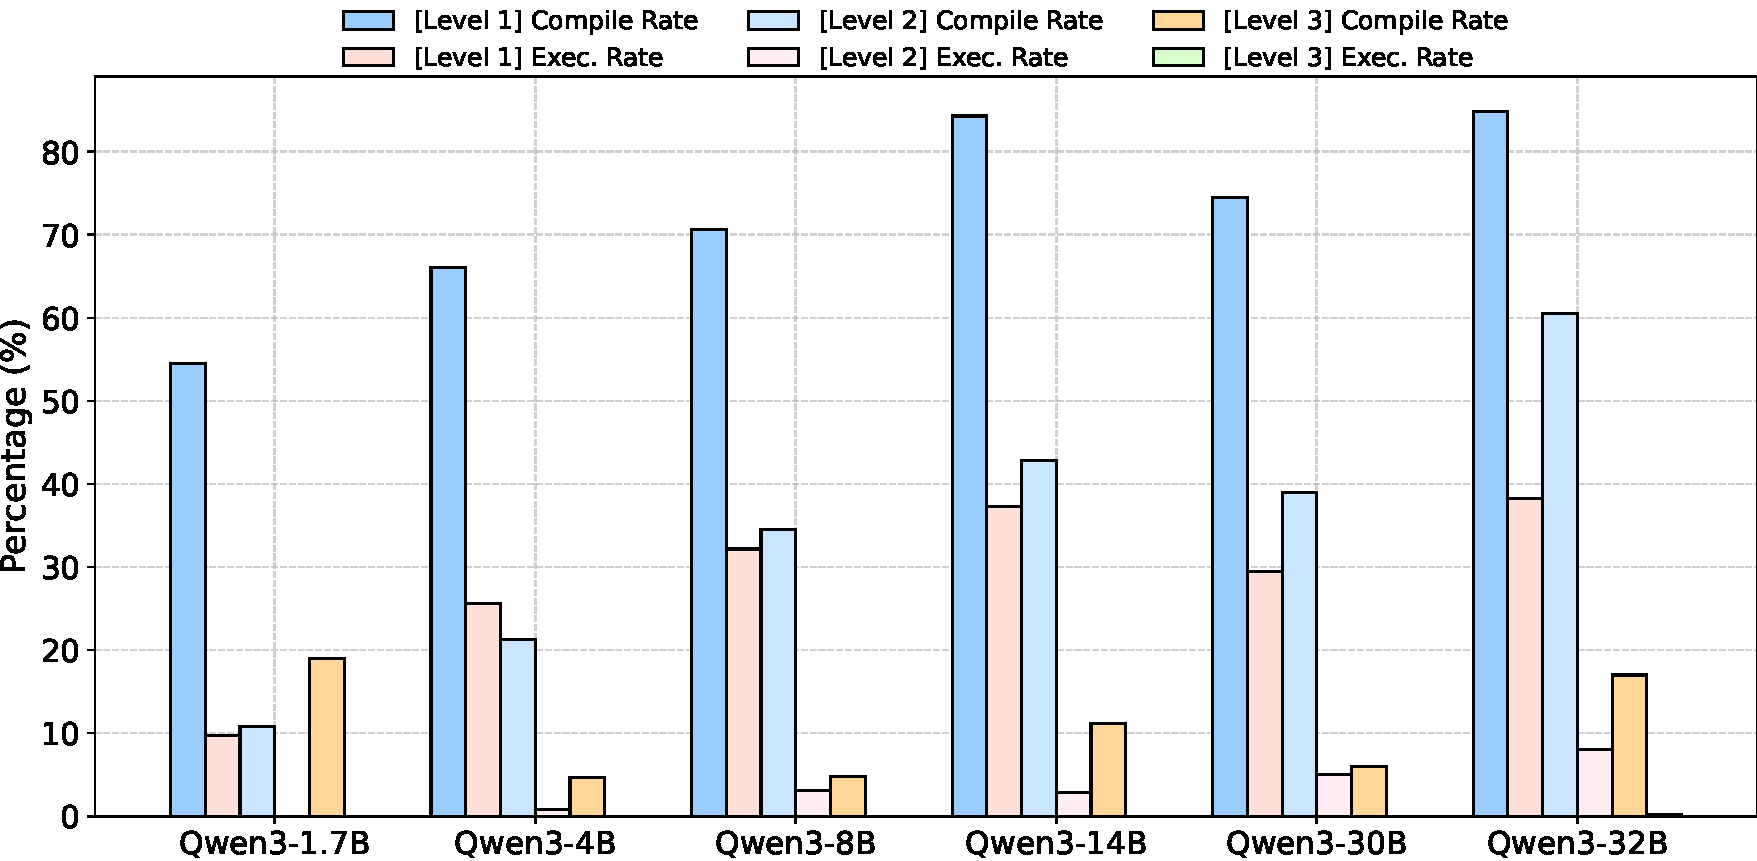
\includegraphics[width=1\linewidth]{pdfs/model_scale.pdf}
    \caption{Scaling behavior of KernelGen-LM on NPU kernel generation tasks with increasing difficulty.}
    \label{fig:model_scale}
\end{figure}

As shown in Figure~\ref{fig:model_scale}, increasing model scale leads to clear performance gains on Level~1 and Level~2 tasks, indicating that larger models better capture standard kernel patterns. In contrast, Level~3 tasks remain highly challenging, with most models failing to achieve non-trivial execution rates. However, 32B is the only scale that demonstrates measurable compilation success on Level~3, suggesting that sufficient parameter scale is a prerequisite for reasoning over the complex control flow and memory dependencies of complicated NPU kernels.

\subsubsection{Comparison of Fine-tuning Strategies}  
% 全量微调与 LoRA 微调策略对比
\begin{table}[t]
    \centering
    \caption{Full-tuning \textit{V.S.} LoRA-tuning in QWen3-8B model.}
    \resizebox{0.75\linewidth}{!}{
    \begin{tabular}{l cc c c}
            \toprule
            \textbf{Model} & \textbf{Level} & \textbf{Compile Rate (\%)} & \textbf{Exec. Rate (\%)} & \textbf{Speedup ($\times$)} \\
            \midrule
            \multirow{4}{*}{LoRA-tuning}  & Level 1   & 54.94 & 20.10  & 0.48 \\  
            & Level 2    & 14.58 & 0.67   & 0.52 \\  
            & Level 3    & 3.83  & 0.00   & - \\ 
            \rowcolor{bggreen}
            & Mean       & 40.29 & 13.55  & 0.48 \\ \hline
             \multirow{4}{*}{Full-tuning}      & Level 1    & 70.67 & 32.17 & 0.58 \\
            & Level 2    & 34.50 & 3.08  & 2.77 \\ 
            & Level 3    & 4.83  & 0.00  & - \\ 
            \rowcolor{bggreen}
            & Mean       & \textbf{55.32} & \textbf{22.13} & \textbf{0.95} \\ 
            \bottomrule
        \end{tabular}
    \label{tab:full_vs_lora}}
\end{table}


Table~\ref{tab:full_vs_lora} compares a comparative analysis between full fine-tuning and LoRA-based fine-tuning on Qwen3-8B.
Full fine-tuning consistently outperforms LoRA across all kernel complexity levels, with the mean compilation rate surging from 40.29\% to 55.32\% and the execution rate improving from 13.55\% to 22.13\%.
The performance gap widens significantly as kernel complexity increases.
We attribute this divergence to the nature of NPU kernel generation, which is a knowledge-intensive task involving strict hardware intrinsics and memory constraints, rather than a simple style transfer.
While LoRA is effective for format alignment, its low-rank decomposition limits the capacity to absorb such high-dimensional, domain-specific knowledge.
In contrast, full fine-tuning updates the entire parameter space, allowing for the deep injection of complex semantics and logical dependencies required for valid code generation.
Consequently, in terms of runtime efficiency, full fine-tuning achieves an average speedup of $0.95\times$, substantially surpassing the $0.48\times$ of LoRA.
These results suggest that for precision-critical tasks like hardware-aware code generation, the comprehensive parameter update of full fine-tuning is indispensable.

\subsubsection{Training Data Composition Analysis} 
% 不同语料来源及数据比例对性能的影响
\begin{figure}[t]
    \centering
    \begin{subfigure}{0.552\textwidth}
        \centering
        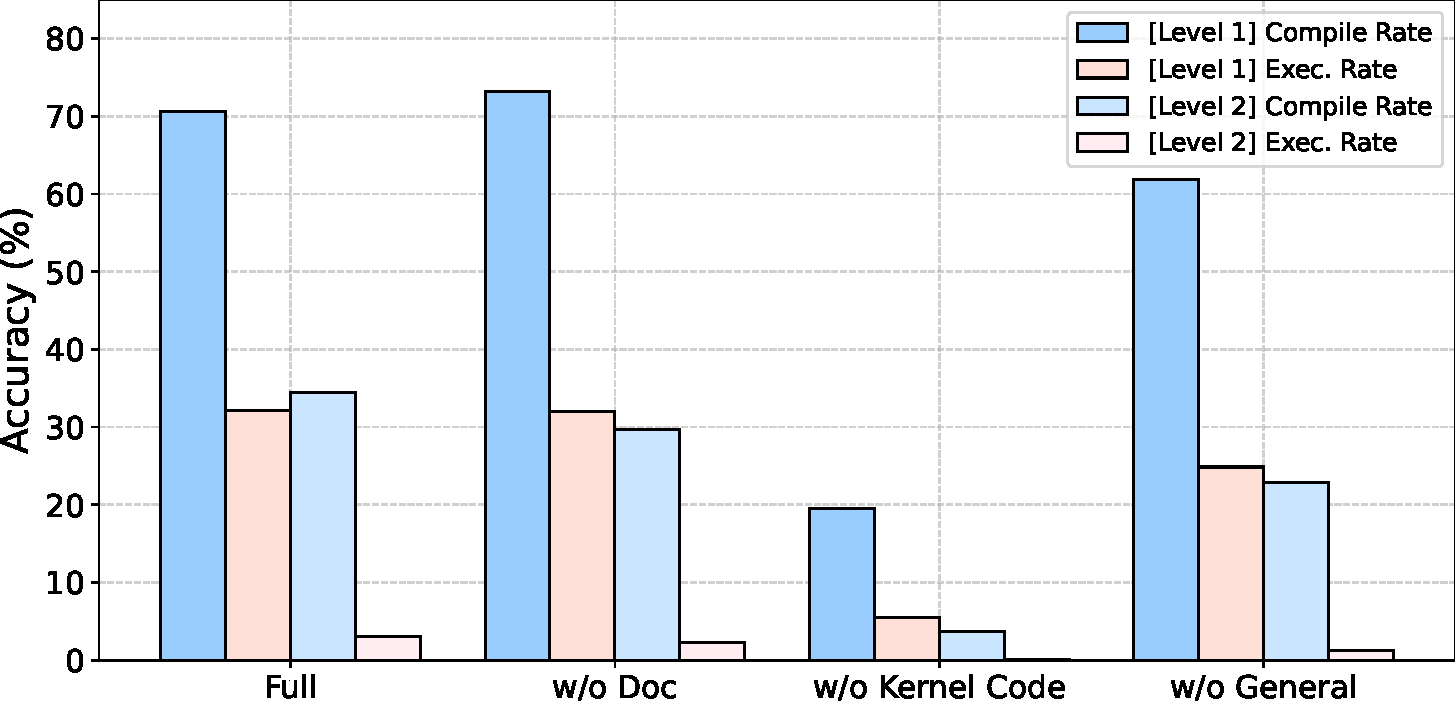
\includegraphics[width=\linewidth]{pdfs/ablation_data_compos.pdf}
        \caption{Pass@1 rates with different data compositions.}
        \label{fig:data_compos}
    \end{subfigure}
    \hfill
    \begin{subfigure}{0.438\textwidth}
        \centering
        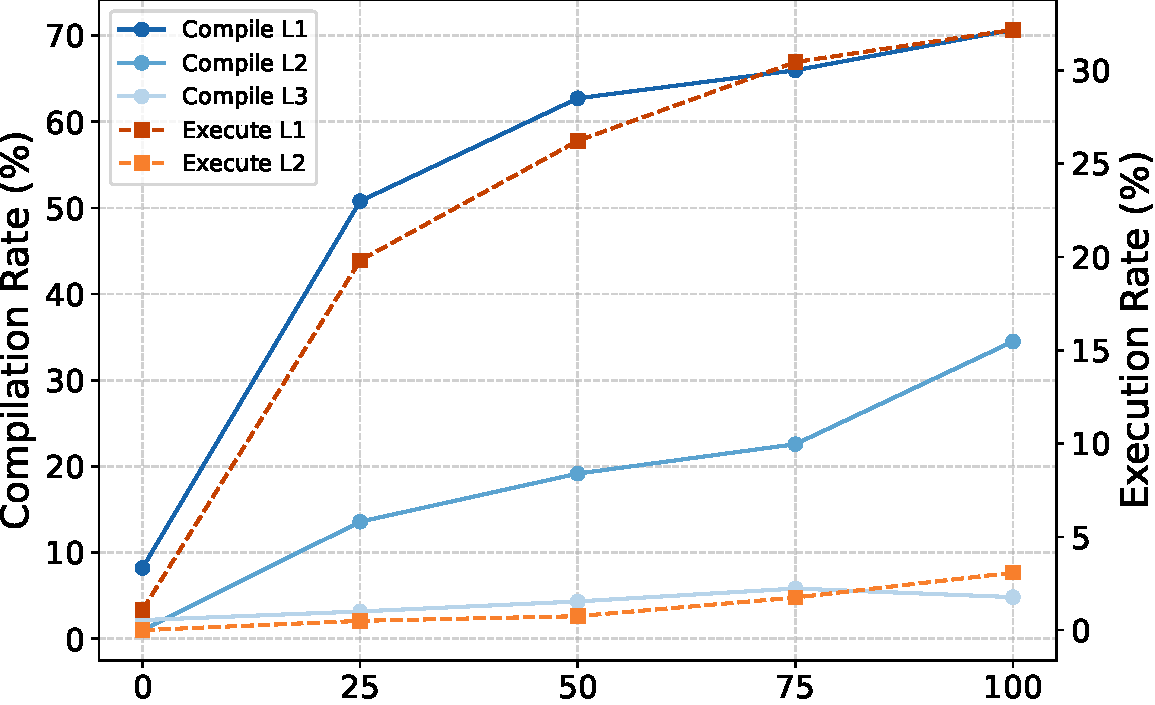
\includegraphics[width=\linewidth]{pdfs/ablation_acc_percent.pdf}
        \caption{Pass@1 rates with varying data ratios in Full setting.}
        \label{fig:data_percent}
    \end{subfigure}
    \caption{Ablation results on training data composition. 
(a) Pass@1 compilation and execution rates for Level~1 and Level~2 kernels on Qwen3-8B under different data composition settings. Removing kernel code leads to the most severe performance degradation, particularly for Level~2 kernels.
(b) Pass@1 compilation and execution rates under the full data setting with different data ratios. Increasing the training data consistently improves both compilation and execution performance.}
    \label{fig:ablation}
\end{figure}

Fig.~\ref{fig:data_compos} shows that removing kernel code from the training data results in a dramatic drop in Pass@1 performance, underscoring its critical role.
Documentation and general semantic data provide auxiliary benefits, particularly for higher-complexity kernels.
Fig.~\ref{fig:data_percent} further demonstrates that increasing the training data size yields consistent improvements, highlighting the importance of data scale.


\subsection{Ablation Analysis of Reinforcement Learning}

\begin{table}[t]
\centering
\caption{DPO hyperparameter ablation in QWen3-8B.}
\resizebox{1\linewidth}{!}{
\begin{tabular}{l c c c c c c}
\toprule
\textbf{Negative Strategy} & \textbf{LR} & \textbf{LR Decay} & \textbf{Batch Size} & \textbf{Training Steps} & \textbf{Compile Rate (\%)} & \textbf{Exec. Rate (\%)} \\
\midrule
 (SFT) & - & - & - & - & \textbf{60.97} & \textbf{5.18}  \\
 \multirow{2}{*}{Compile-pass but execution-fail} 
  &  1e-6 &  constant &  64 &  150 & \textbf{44.21} & \textbf{8.31} \\
  % &  5e-7 &  constant &  128 &  75  & \textbf{56.92}  & \textbf{9.10}  \\
  & 1e-6 &  cosine &  64 &  150  & \textbf{54.03}  & \textbf{9.49}  \\
 Compile-fail &  1e-6 &  constant &  64 &  150 & \textbf{32.00}  & \textbf{6.10} \\
\bottomrule
\end{tabular}
}
\label{tab:DPO_hyper}
\end{table}


Table~\ref{tab:DPO_hyper} presents an ablation study on RL training with different negative strategies and optimization settings, where the negative strategies follow the preference data construction introduced in Sec.~\ref{reinforcement_learning}. Comparing the second row (compile-pass but execution-fail) with the fourth row (compile-fail) shows that using execution-failed yet compilation-passed samples as negatives leads to markedly better compilation and execution performance, indicating that such preference data provides more informative supervision than compile-failed negatives. Under the same negative strategy, a further comparison between the second and third rows demonstrates that cosine learning rate decay consistently outperforms a constant schedule, especially in terms of execution success. These results jointly motivate our choice of execution-failed but compilation-passed samples as negative preferences and cosine decay as the default optimization setting for RL training.

\subsection{Error Analysis}

To better understand the limitations of LLM-based kernel generation, we conduct a systematic error analysis over approximately 4,000 failed kernel generations.
Figure~\ref{fig:placeholder} summarizes the distribution of observed failure types.


\begin{wrapfigure}{r}{0.45\linewidth}
    \centering
    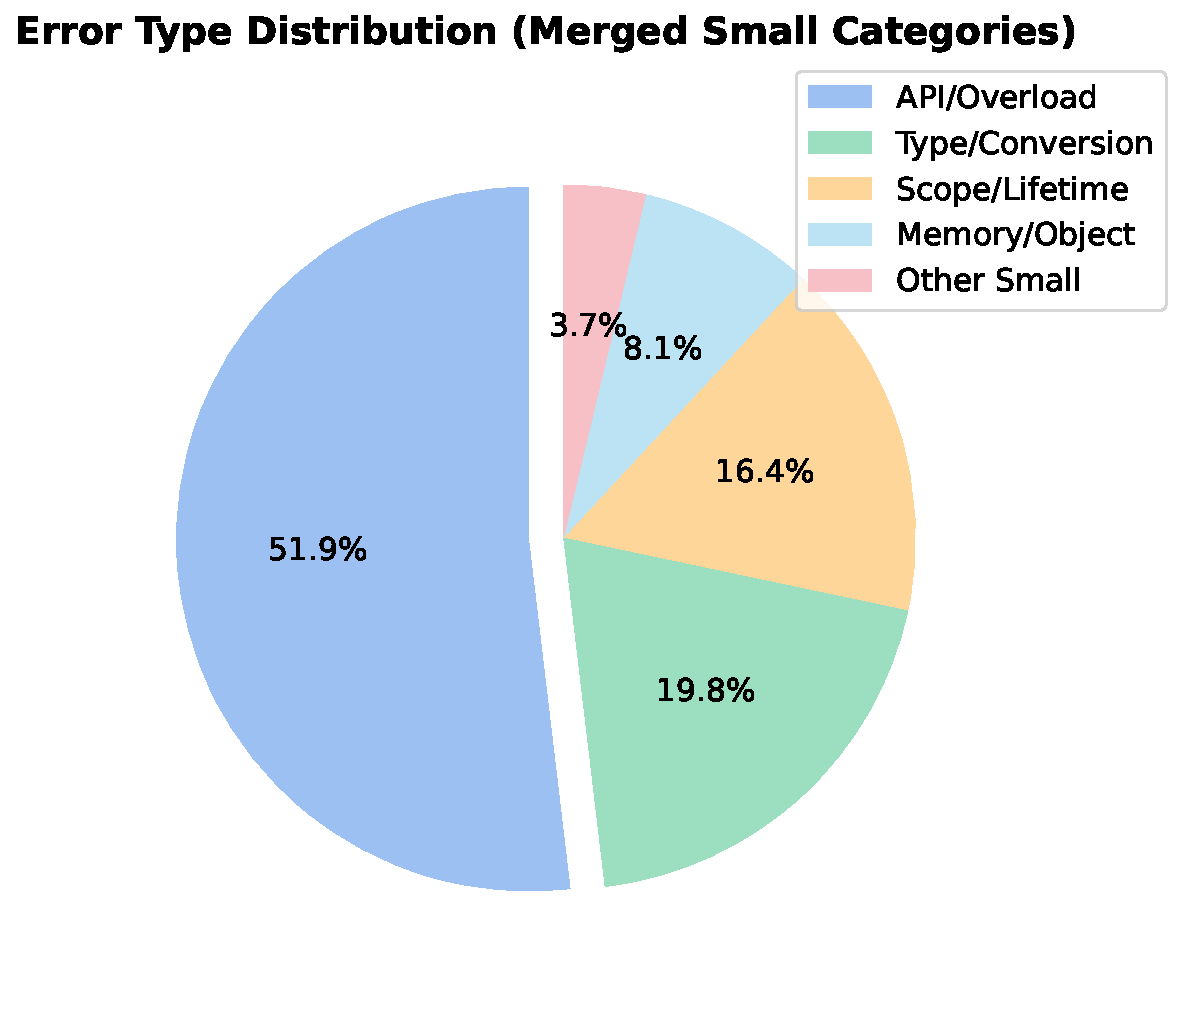
\includegraphics[width=\linewidth]{pdfs/ablation_error_type.pdf}
    \caption{Distribution of kernel generation errors.}
    \label{fig:placeholder}
\end{wrapfigure}

\begin{comment}

Data Type \& Conversion Errors follow, representing 19.8\% of failures and typically arising from type inconsistencies, invalid casting, or shape mismatches.
Variable Scope \& Lifetime Errors constitute 16.4\% of failures, reflecting challenges in correctly managing intermediate buffers, variable lifetimes, and temporary objects.
Finally, the remaining low-frequency errors, including memory \& object usage, syntax \& structure, and macro \& preprocessing errors (combined 3.7\%), are grouped as Other Errors.

\end{comment}

%API Signature and Overload Errors are the most frequent, accounting for 51.9\% of failures, followed by Data Type and Conversion Errors (19.8\%) and Variable Scope and Lifetime Errors (16.4\%). Lower-frequency errors, including memory usage, syntax, and macro-related issues, together account for 3.7\%. These results indicate that while structural and memory-related issues are relatively well handled, generating correct API calls and managing data types and variable scope remain significant challenges for current models.

As shown in the figure, API Signature and Overload Errors constitute the dominant failure mode, accounting for 51.9\% of all failed cases. These errors occur when generated function invocations fail to match any valid AscendC API signature or overload. The second most common category is Data Type and Conversion Errors (19.8\%), followed by Variable Scope and Lifetime Errors (16.4\%) and Memory and Object Usage Errors (8.1\%). Lower-frequency failures—including syntax and structural violations as well as macro and preprocessing errors—together account for only 3.7\% of all cases.

\begin{comment}

The most prevalent failure mode corresponds to API signature and overload errors, accounting for 51.9\% of all failures.
These errors arise when generated function invocations do not match any valid AscendC API signature.
The next most frequent categories include data type and conversion errors (19.8\%) and variable scope and lifetime errors (16.4\%).
In contrast, errors related to syntax, memory usage, and macro preprocessing are relatively rare, jointly contributing only 3.7\% of the total failures.

This distribution reveals a clear pattern: while current models are generally capable of producing syntactically valid kernel structures and managing basic memory operations, they struggle with semantically constrained reasoning, particularly in API invocation, type consistency, and program state management.

\end{comment}

%In the following, we analyze the major error categories to understand their underlying causes and implications for LLM-based kernel generation.
%Overall, the observed failures can be grouped into three high-level error modes, reflecting limitations in API reasoning, low-level type handling, and program state management.

This distribution indicates that current models are generally capable of producing syntactically well-formed kernel code, as purely syntactic and structural errors are relatively rare.
However, the majority of failures arise from semantically constrained aspects of low-level programming.
In particular, errors are dominated by cases that require precise reasoning about API contracts, hardware-specific data types, and variable visibility across different kernel components.

To further investigate the underlying causes of these failures, we analyze the major error categories in detail. Below, we describe each error category along with its typical causes and manifestations.

\begin{comment}

Based on these observations, we cluster the failures into three high-level error modes that reflect fundamental reasoning limitations in low-level kernel generation.
First, \emph{API reasoning errors} occur when the model fails to align function arguments with hardware-specific API contracts, leading to invalid overload resolution.
Second, \emph{type-level reasoning errors} stem from improper handling of low-level data types and implicit conversions, which are especially error-prone in performance-critical kernel code.
Third, \emph{program state management errors} arise from incorrect assumptions about variable scope, lifetime, or visibility across host–kernel boundaries.

Less frequent failure modes, including memory object misuse, syntactic inconsistencies, and macro-related issues, can be largely attributed to incomplete code generation or template misalignment rather than fundamental reasoning gaps.
Representative examples of each error category are provided in Table~\ref{tab:error_examples} in the Appendix.

\end{comment}

\begin{itemize}
    \item \textbf{API Signature \& Overload Errors}: These errors arise when a generated function call does not match any valid API signature or overload defined in the programming interface. Common causes include incorrect argument ordering, mismatched parameter types, missing required parameters, or confusion between similarly named APIs with subtle semantic differences. This category reflects the model’s difficulty in aligning high-level task intent with rigid, hardware-specific API contracts.
    
    \item \textbf{Data Type \& Conversion Errors}: This category includes the use of invalid or non-existent data types (e.g., \texttt{bool\_t}), as well as illegal or unsafe type conversions between incompatible types (e.g., mixing \texttt{float} and \texttt{double} constants). Such errors often stem from implicit assumptions carried over from high-level programming languages, which do not hold in low-level kernel development where type rules are strict and hardware-dependent.

    \item \textbf{Variable Scope \& Lifetime Errors}: These errors occur when variables are used outside their valid scope or before being properly defined. Typical examples include references to undeclared symbols (e.g., \texttt{M\_PI}) or misuse of variables that are not visible within the current compilation unit or kernel context. This category highlights challenges in consistently reasoning about variable visibility and lifetime across host-side logic, kernel code, and auxiliary configuration structures.
    
    \item \textbf{Memory \& Object Usage Errors}: Errors in this category are related to incorrect usage of core objects such as \texttt{TPipe}, \texttt{LocalTensor}, and \texttt{GlobalTensor}. They include invalid member function invocations and incorrect memory address computations. While less frequent, such errors can lead to severe runtime failures or undefined behavior.

    \item \textbf{Syntax \& Structure Errors}: These errors stem from violations of C++ syntax or incomplete kernel class definitions. Examples include missing required methods (e.g., improperly defined or absent \texttt{Init} functions), mismatched braces, or malformed template instantiations.
    These errors are typically associated with incomplete code generation rather than deeper semantic misunderstandings.

    \item \textbf{Macro \& Preprocessing Errors}: This category includes errors caused by incorrect macro definitions or improper usage of tiling-related preprocessing directives. These issues often arise from incorrect assumptions about compile-time constants or conditional compilation logic embedded in kernel templates.

\end{itemize}

\begin{comment}

\begin{itemize}
    \item \textbf{API-Level Reasoning Errors.}
    The most prevalent failures arise from incorrect API usage, including signature mismatches and overload resolution errors.
    Although the generated code often appears syntactically plausible, the arguments do not conform to any valid API signature.
    This indicates that current models struggle to precisely align function semantics with hardware-specific API contracts.

    \item \textbf{Type System and Data Representation Errors.}
    A substantial portion of failures are caused by invalid data types or illegal type conversions, such as the use of unsupported types (e.g., \texttt{bool\_t}) or inconsistent constant types (\texttt{float} vs.\ \texttt{double}).
    These errors suggest limited robustness in modeling low-level type systems and numeric constraints imposed by NPU kernels.

    \item \textbf{Program State and Structural Errors.}
    The remaining failures are related to incorrect management of program state, including variable scope and lifetime errors, improper memory or object usage involving \texttt{TPipe}, \texttt{LocalTensor}, and \texttt{GlobalTensor}, as well as syntax, class structure, and macro preprocessing issues.
    While individually less frequent, these errors highlight challenges in generating globally consistent and executable kernel programs.
\end{itemize}

\end{comment}

Representative examples for each error category are provided in Table~\ref{tab:error_examples} in the Appendix.